\subsection{Interpolation}

\frame{\tableofcontents[currentsubsection]}

\begin{frame}
  \frametitle{Interpolation}
  \begin{center}
    \begin{tikzpicture}[milestone/.style={drop shadow,draw,fill=red!50,minimum height=7.5mm,minimum width=1cm,font=\tiny\scshape},
                        link/.style={-latex,thick},
                        arrow/.style={blue,ultra thick,-{Stealth[]}},
                        scale=.8,transform shape]
      \node[milestone] (uint8) at (0,0) {\texttt{Stream<uint8>}};
      \node[milestone] (int16) at ($ (uint8) + (2,1) $) {\texttt{Stream<int16>}};
      \node[milestone] (double) at ($ (uint8) + (4,0) $) {\texttt{Stream<double>}};
      \node[milestone] (wave) at ($ (double) + (3,0) $) {\texttt{Wave}};

      \draw[link] (uint8) |- (int16);
      \draw[link] (int16) -| (double);
      \draw[link] (uint8) -- (double);
      \draw[link] (double) -- (wave);

      
      \coordinate (link middle) at ($ (double.east) ! 0.5 ! (wave.west) $);
      \draw[arrow] ($ (link middle) - (0,1.5) $) -- (link middle);
    \end{tikzpicture}
  \end{center}
  \begin{itemize}
    \item \texttt{Stream<double>} is a sequence of discrete values (red)
    \item We want to construct a continuous curve (blue)
  \end{itemize}
  \begin{center}
    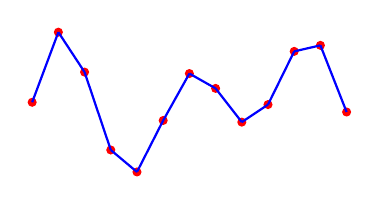
\begin{tikzpicture}
      \draw[fill,red] (0,0) circle [radius=0.05cm];
      \foreach[count=\i,
               evaluate={sin(2.5*\x) * 0.6 + cos(1.3*\x) * 0.4} as \y,
               remember=\y as \lasty (initially 0),
               remember=\x as \lastx (initially 0)] \x in {30,60,...,360} {
        \draw[fill,red] (\x*0.0111,\y) circle [radius=0.05cm];
        \draw[thick,blue] (\lastx*0.0111,\lasty) -- (\x*0.0111,\y);
      }
    \end{tikzpicture}
  \end{center}
\end{frame}

\begin{frame}
  \frametitle{Interpolation}
  \begin{itemize}
    \item Connecting dots is also called \emph{interpolation}
    \item Formula to connect $(x_1,y_1)$ with $(x_2,y_2)$ is
          \[
            y = m \cdot x + q
          \]
          with
          \[
            \begin{array}{rcl}
              m & = & \displaystyle \frac{y_2-y_1}{x_2-y_1} \\ \\
              q & = & \displaystyle \frac{x_2 y_1-x_1y_2}{x_2-x_1} \\
            \end{array}
          \]
    \item We need to draw many such segments
  \end{itemize}
\end{frame}



%%% Local Variables:
%%% mode: latex
%%% TeX-master: "sound"
%%% End:
